\documentclass[aspectratio=1610]{beamer}

\usetheme{Boadilla}

\usepackage{todonotes}
\setuptodonotes{inline} % need this, because beamer slides don't have a margin

\usepackage[utf8]{inputenc}
\usepackage[T1]{fontenc}
\usepackage{lmodern}
\usepackage{graphicx}
\usepackage{booktabs}
\usepackage{listings}
\usepackage{xcolor}
\usepackage{hyperref}
\usepackage{csquotes}
\usepackage{tikz}
\usetikzlibrary{arrows.meta, positioning}

\graphicspath{{../00_Bilder/}}

% Anpassung der Kopfzeile, um die aktuelle section und subsection anzuzeigen
\setbeamertemplate{headline}{
	\leavevmode%
	\hbox{%
		\begin{beamercolorbox}[wd=.5\paperwidth,ht=2.5ex,dp=1.125ex,left]{section in head/foot}%
			\usebeamerfont{section in head/foot}\hspace*{0.2cm}\insertsectionhead\hspace*{2ex}
		\end{beamercolorbox}%
		\begin{beamercolorbox}[wd=.5\paperwidth,ht=2.5ex,dp=1.125ex,right]{subsection in head/foot}%
			\usebeamerfont{subsection in head/foot}\hspace*{2ex}\insertsubsectionhead
		\end{beamercolorbox}
	}%
	\vskip0pt%
}

\setbeamertemplate{footline}
{
	\leavevmode%
	\hbox{%
		\begin{beamercolorbox}[wd=.333333\paperwidth,ht=2.25ex,dp=1ex,center]{author in head/foot}%
			\usebeamerfont{author in head/foot}\insertshortauthor
		\end{beamercolorbox}%
		\begin{beamercolorbox}[wd=.333333\paperwidth,ht=2.25ex,dp=1ex,center]{title in head/foot}%
			\usebeamerfont{title in head/foot}\insertshorttitle
		\end{beamercolorbox}%
		\begin{beamercolorbox}[wd=.333333\paperwidth,ht=2.25ex,dp=1ex,right]{date in head/foot}%
			\usebeamerfont{date in head/foot}\insertshortdate{}\hspace*{2em}
			\insertframenumber{} / \inserttotalframenumber\hspace*{2ex} 
	\end{beamercolorbox}}%
	\vskip0pt%
}

\definecolor{codegray}{RGB}{40,40,40}
\definecolor{codebg}{RGB}{245,245,245}

\lstdefinelanguage{JSON}{
	basicstyle=\ttfamily\small,
	literate=
	*{0}{{{\color{blue}0}}}{1}
	{1}{{{\color{blue}1}}}{1}
	{2}{{{\color{blue}2}}}{1}
	{3}{{{\color{blue}3}}}{1}
	{4}{{{\color{blue}4}}}{1}
	{5}{{{\color{blue}5}}}{1}
	{6}{{{\color{blue}6}}}{1}
	{7}{{{\color{blue}7}}}{1}
	{8}{{{\color{blue}8}}}{1}
	{9}{{{\color{blue}9}}}{1}
	{:}{{{\color{black}{:}}}}{1}
	{,}{{{\color{black}{,}}}}{1}
	{"}{{{\color{red}{"}}}}{1},
	showstringspaces=false,
	backgroundcolor=\color{codebg},
	frame=single
}

\lstdefinelanguage{HTTP}{
	basicstyle=\ttfamily\small,
	morekeywords={GET,POST,PUT,DELETE,HTTP},
	backgroundcolor=\color{codebg},
	frame=single
}

\lstdefinelanguage{JavaScript}{
	basicstyle=\ttfamily\small,
	keywords={const,let,var,async,await,fetch,then},
	backgroundcolor=\color{codebg},
	frame=single
}

\title[Standards \& AI]{Standards, FHIR \& AI in Healthcare}
\subtitle{Workshop UPNA 2026 -- Day 2}
\author{Prof. Dr. Rafael Mayoral Malmström}
\institute[Kempten UAS]{Hochschule Kempten -- University of Applied Sciences}
\date{Spring 2026}

\titlegraphic{%
	\hfill
	\raisebox{-0.5\height}{%
		\begin{minipage}{6cm}
			\centering
			
\includegraphics[height=1.3cm]{kempten_IF_logo.png}
			\hspace{0.3cm}
			
\includegraphics[height=1.1cm]{Logo_UPNA.svg}
			
			\par\vspace{0.2cm} % spacing between logos and slogan
			\tiny\textit{Erasmus+ Teaching Mobility 2026}
		\end{minipage}
	}%
}

\begin{document}
	
	%=====================================================
	\begin{frame}
		\titlepage
	\end{frame}
	
	%=====================================================
	\begin{frame}{Agenda -- Day 2}
		\begin{enumerate}
			\item Recap of Day 1
			\item Web app + FHIR demo
			\item Standards and AI in healthcare (mini-module)
			\item Group activity: design your own FHIR-based use case
			\item Lightning presentations \& wrap-up
		\end{enumerate}
	\end{frame}
	
	%=====================================================
	\section{Recap}
	
	\begin{frame}{Day 1 Recap}
		\begin{itemize}
			\item FHIR basics: resources, references, JSON representation
			\item RESTful operations: GET, POST, PUT, DELETE
			\item Lab 1: creating Patients and Observations
			\item Lab 2: mini workflow with DiagnosticReport
		\end{itemize}
		\vspace{0.5em}
		\begin{block}{Today}
			\begin{itemize}
				\item See how a web app talks to FHIR
				\item Understand why standards matter for AI
				\item Design your own FHIR-based mini solution
			\end{itemize}
		\end{block}
	\end{frame}
	
	%=====================================================
	\section{Web App + FHIR}
	
	\begin{frame}{From Notebook to Web App}
		\begin{itemize}
			\item Yesterday: direct HTTP requests via Python/Colab
			\item Today: simple web client (browser) calling FHIR server
			\item Same REST endpoints, different client
		\end{itemize}
		% TODO: add diagram: Browser (JS) -> FHIR API -> Server -> JSON -> Browser UI
	\end{frame}
	
	
	\begin{frame}{From Browser UI to FHIR Server (Architecture Overview)}
		\vspace{0.2cm}
		
		\begin{center}
			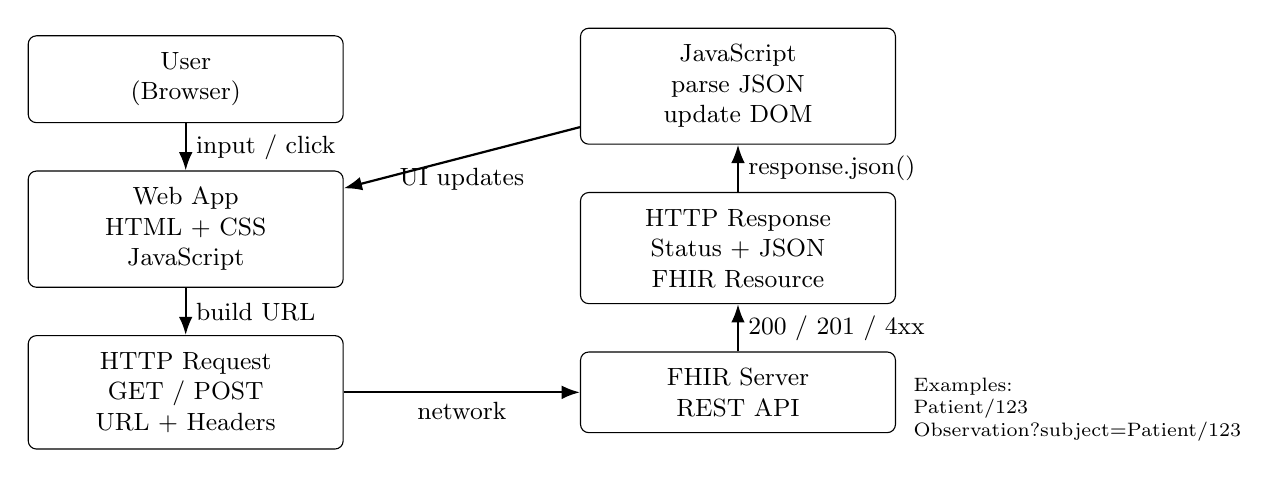
\begin{tikzpicture}[
				font=\small,
				node distance=6mm and 9mm,
				box/.style={draw, rounded corners=3pt, align=center, inner sep=6pt, minimum width=4.0cm},
				arrow/.style={-Latex, thick}
				]
				
				% Nodes
				\node[box] (user) {User\\(Browser)};
				\node[box, below=of user] (ui) {Web App\\HTML + CSS\\JavaScript};
				\node[box, below=of ui] (http) {HTTP Request\\GET / POST\\URL + Headers};
				\node[box, right=3.0cm of http] (server) {FHIR Server\\REST API};
				\node[box, above=of server] (json) {HTTP Response\\Status + JSON\\FHIR Resource};
				\node[box, above=of json] (render) {JavaScript\\parse JSON\\update DOM};
				
				% Arrows (downstream)
				\draw[arrow] (user) -- node[right]{input / click} (ui);
				\draw[arrow] (ui) -- node[right]{build URL} (http);
				\draw[arrow] (http) -- node[below]{network} (server);
				
				% Arrows (upstream)
				\draw[arrow] (server) -- node[right]{200 / 201 / 4xx} (json);
				\draw[arrow] (json) -- node[right]{response.json()} (render);
				\draw[arrow] (render) -- node[below]{UI updates} (ui);
				
				% Optional callouts
				\node[align=left, font=\scriptsize, anchor=west] at ([xshift=0.1cm,yshift=0.3cm]server.south east) {Examples:\\Patient/123\\Observation?subject=Patient/123};
				
			\end{tikzpicture}
		\end{center}
		
		\vspace{0.2cm}
		\begin{itemize}
			\item \textbf{Same mental model as Day 1:} URL + HTTP method + JSON
			\item \textbf{FHIR adds semantics:} resource types, references, codes (e.g., LOINC)
			\item \textbf{Tomorrow's focus:} turning REST calls into an interactive UI
		\end{itemize}
		
	\end{frame}
	
	
	
	%=====================================================
\begin{frame}[fragile]{Minimal JavaScript Example}
	
	\lstset{
		language=JavaScript,
		basicstyle=\ttfamily\scriptsize,  % smaller font
		breaklines=true,                   % automatically wrap long lines
		breakatwhitespace=true
	}
	
	\begin{lstlisting}
const FHIR_SERVER = "https://example.org/fhir/";
		
async function loadPatient(patientId) {
	const response = await fetch(
	FHIR_SERVER + "Patient/" + patientId,
	{ headers: { "Accept": "application/fhir+json" } }
	);
	const data = await response.json();
	console.log(data);
}
	\end{lstlisting}
	
	\begin{itemize}
		\item Called from HTML (e.g., button click)
		\item Shows how UI, JavaScript, and FHIR connect
	\end{itemize}
	
\end{frame}
	
	%=====================================================
	\begin{frame}[fragile]{Simple UI Sketch (Conceptual)}
		\begin{itemize}
			\item Input: Patient ID
			\item Button: ``Load patient''
			\item Display: patient name, birthdate, list of Observations
		\end{itemize}
		% TODO: add a simple wireframe: text field + button + data area
	\end{frame}
	
	%=====================================================
	\begin{frame}{Key Takeaways: Web Clients}
		\begin{itemize}
			\item Browser acts as FHIR client
			\item REST endpoints remain the same
			\item Security (auth, HTTPS, tokens) is critical in real systems
			\item Today: we focus on data flow, not on full security model
		\end{itemize}
	\end{frame}
	
	%=====================================================
	\section{Standards \& AI in Healthcare}
	
	\begin{frame}{Why AI Needs Good Data}
		\begin{itemize}
			\item Machine learning models rely on:
			\begin{itemize}
				\item large amounts of data
				\item consistent structure
				\item correct semantics
			\end{itemize}
			\item Garbage in, garbage out:
			\begin{itemize}
				\item inconsistent coding
				\item missing values
				\item ambiguous meaning
			\end{itemize}
			\item Standards help address these issues
		\end{itemize}
	\end{frame}
	
	%=====================================================
	\begin{frame}{Role of Standards (FHIR, Terminologies)}
		\begin{itemize}
			\item FHIR standardizes \textbf{structure} and \textbf{syntax}:
			\begin{itemize}
				\item JSON layout
				\item resource fields
				\item references
			\end{itemize}
			\item Terminologies standardize \textbf{meaning}:
			\begin{itemize}
				\item LOINC for measurements
				\item SNOMED CT for clinical concepts
				\item ICD for diagnoses (administrative)
			\end{itemize}
			\item Together: \textbf{semantic interoperability} $\rightarrow$ more reliable data for AI and analytics
		\end{itemize}
	\end{frame}
	
	%=====================================================
	\begin{frame}{Example: Vital Signs for Risk Prediction}
		\begin{itemize}
			\item Data sources:
			\begin{itemize}
				\item Observations of blood pressure, heart rate, temperature
			\end{itemize}
			\item Standard coding:
			\begin{itemize}
				\item LOINC codes for each measurement
			\end{itemize}
			\item FHIR Observations provide:
			\begin{itemize}
				\item numeric values
				\item units
				\item timestamps
				\item patient reference
			\end{itemize}
			\item AI-friendly dataset:
			\begin{itemize}
				\item features: latest BP, average HR, etc.
				\item labels: outcome (e.g., ICU admission, complication)
			\end{itemize}
		\end{itemize}
	\end{frame}
	
	%=====================================================
	\begin{frame}{From FHIR to Feature Table (Conceptual)}
		\begin{itemize}
			\item Step 1: extract Observations from FHIR server
			\item Step 2: filter by code and time
			\item Step 3: aggregate (mean, max, last value)
			\item Step 4: build a row per patient:
			\begin{itemize}
				\item columns = features
			\end{itemize}
			\item Step 5: feed into ML model
		\end{itemize}
		% TODO: add diagram: FHIR resources → ETL → tabular data → model
	\end{frame}
	
	%=====================================================
	\begin{frame}[fragile]{Toy Example: Simple Rule on FHIR Data}
		\lstset{language=JSON}
		\begin{lstlisting}
{
	"resourceType": "Observation",
	"status": "final",
	"code": { ... },
	"subject": { "reference": "Patient/123" },
	"valueQuantity": { "value": 160, "unit": "mmHg" }
}
		\end{lstlisting}
		
		\begin{itemize}
			\item Simple rule-based logic (not full AI!):
			\begin{itemize}
				\item If systolic BP > 140 mmHg $\rightarrow$ ``high blood pressure alert''
			\end{itemize}
			\item Demonstrates how structured FHIR data can drive simple decision rules
		\end{itemize}
	\end{frame}
	
	%=====================================================
	\begin{frame}{Trustworthy AI in Healthcare (High-Level)}
		\begin{itemize}
			\item Beyond technical performance:
			\begin{itemize}
				\item Transparency: Decisions and data sources must be understandable
				\item Fairness: Performance should not systematically disadvantage patient groups
				\item Robustness: Results must remain reliable under imperfect conditions
				\item Accountability: Clear responsibility must exist for system outcomes
			\end{itemize}
			\item Standards contribute to:
			\begin{itemize}
				\item Traceability of input data
				\item Consistent meaning across systems
				\item Better documentation of data provenance
			\end{itemize}
			\item Regulatory frameworks (e.g., EU AI Act) emphasize data quality and governance
		\end{itemize}
	\end{frame}
	
	%=====================================================
	\section{Group Activity}
	
	\begin{frame}{Group Activity: FHIR-Based Mini Use Case}
		\begin{block}{Task (in teams of 2--3)}
			\begin{itemize}
				\item Choose a clinical scenario
				\item Identify FHIR resources needed
				\item Decide which REST operations are used
				\item Sketch the user interface
				\item Optionally add a simple alert rule
			\end{itemize}
		\end{block}
	\end{frame}
	
	%=====================================================
	\begin{frame}{Example Scenario: Hypertension Monitoring}
		\begin{itemize}
			\item Scenario:
			\begin{itemize}
				\item Patient measures BP at home
				\item Values are stored as Observations
				\item Clinician receives a summary (DiagnosticReport)
			\end{itemize}
			\item FHIR resources:
			\begin{itemize}
				\item \texttt{Patient}, \texttt{Observation}, \texttt{DiagnosticReport}
			\end{itemize}
			\item REST operations:
			\begin{itemize}
				\item \texttt{POST /Observation}
				\item \texttt{GET /Observation?subject=Patient/123}
			\end{itemize}
			\item Optional alert:
			\begin{itemize}
				\item If multiple Observations > 160 mmHg $\rightarrow$ flag as ``urgent''
			\end{itemize}
		\end{itemize}
	\end{frame}
	
	%=====================================================
	\begin{frame}{Group Output}
		\begin{itemize}
			\item Use the template provided:
			\begin{itemize}
				\item Clinical scenario (1--2 sentences)
				\item FHIR resources involved
				\item REST operations
				\item UI sketch (very simple)
				\item Optional AI/alert idea
			\end{itemize}
			\item Prepare a 1--2 minute lightning presentation
		\end{itemize}
	\end{frame}
	
	%=====================================================
	\section{References \& Further Reading}
	
	\begin{frame}{Standards \& AI References}
		\small
		\begin{itemize}
			\item HL7 FHIR Official Spec: \url{https://www.hl7.org/fhir/}
			\item LOINC: \url{https://loinc.org/}
			\item SNOMED CT: \url{https://www.snomed.org/}
			\item Overview of AI in healthcare (example introductory sources, adapt as needed):
			\begin{itemize}
				\item Topol, E. \emph{Deep Medicine: How Artificial Intelligence Can Make Healthcare Human Again}.
				\item Short tutorials and review articles from major journals (e.g., NEJM, Lancet Digital Health).
			\end{itemize}
		\end{itemize}
	\end{frame}
	
	%=====================================================
	\begin{frame}{Wrap-Up}
		\begin{itemize}
			\item FHIR and terminologies provide a solid foundation for interoperable data
			\item Web apps and services can use this foundation to build useful tools
			\item AI benefits from high-quality, standardised datasets
			\item You have:
			\begin{itemize}
				\item practiced FHIR/REST in labs
				\item seen a web client in action
				\item designed your own mini use case
			\end{itemize}
		\end{itemize}
		\vspace{0.5em}
		\centering
		\Large Thank you!
	\end{frame}
	
	%=====================================================
	
\end{document}
